\documentclass[10pt,conference]{IEEEtran}
\usepackage{booktabs}
\usepackage{graphicx}
\usepackage{amsmath}
\usepackage{url}
\usepackage[hidelinks]{hyperref}

% DRAFT. Every number in this file must trace to a file under data/, runs/ or
% sim/results/. Placeholders are marked TODO(measured) or TODO(sim). Simulated
% results are always labelled as simulated in the text and captions.

\title{Which Signal Should LLM Inference Scale On?\\
A Controlled Comparison of Reactive Kubernetes Autoscaling Signals\\
Calibrated to Measured vLLM Behavior}
\author{\IEEEauthorblockN{Ruthvik Garlapati}\IEEEauthorblockA{Independent}}

\begin{document}
\maketitle

\begin{abstract}
TODO: write last, after results are final. Shape: problem (operators pick an
autoscaling signal for vLLM on Kubernetes from vendor guidance); what we did
(measured single-replica vLLM on T4 across three sessions and two providers;
compared seven reactive signals plus static provisioning on a kind cluster
with an emulator calibrated to those measurements, and swept control-loop
parameters in a calibrated simulator); top findings with numbers; artifact.
\end{abstract}

\section{Introduction}
Large language model (LLM) inference servers such as vLLM~\cite{kwon2023vllm}
are increasingly deployed on Kubernetes and scaled horizontally by the
Horizontal Pod Autoscaler (HPA)~\cite{k8shpa}, often through KEDA~\cite{keda},
which lets the HPA act on arbitrary Prometheus queries. The operator must
choose which server metric to scale on: queue depth, batch size, KV-cache
usage, a latency signal such as time to first token (TTFT), or request
throughput. Public guidance differs. Cloud documentation recommends queue size
for throughput and batch size for latency-sensitive workloads and warns that
GPU utilization is misleading~\cite{gke2026autoscaling}; project documentation
for llm-d suggests KV-cache utilization thresholds around 0.8. These
recommendations are rarely accompanied by controlled comparisons under the
same workload and the same control loop.

Recent work shows that for LLM serving, the startup delay of a new replica
dominates the outcome of reactive scaling, and that predictive, delay-aware
controllers recover most of the loss~\cite{liu2026decomposing}. Model-based
controllers that predict latency from a queueing model have also been
proposed~\cite{ramani2026queueing}, as have hierarchical and forecast-driven
autoscalers~\cite{patke2025chiron,jaiswal2025sageserve}. These systems are
compared against one or two reactive baselines. What remains unclear for the
operator who deploys the default reactive stack is how the common reactive
signals compare with each other, why each fails when it fails, and how
sensitive each is to the control-loop settings that the operator controls.

This paper answers those questions with a controlled, low-cost, reproducible
methodology. Our contributions are:
\begin{itemize}
\item A measured single-replica profile of vLLM~0.32.0 serving
  Qwen2.5-1.5B-Instruct on an NVIDIA T4, repeated in three sessions on two
  providers, including capacity, the behavior of each candidate scaling
  signal under load, and the distribution of cold-start time
  (Section~\ref{sec:profile}).
\item A comparison of seven reactive scaling policies and static provisioning
  on a real Kubernetes control plane (kind, Prometheus, KEDA, HPA), with the
  server replaced by an emulator calibrated to the measured profile, under
  identical burst and ramp workloads, five trials each
  (Section~\ref{sec:kind}).
\item An analysis of failure mechanisms: a KV-cache signal that cannot reach
  common thresholds when prompts are short, queue-depth overshoot driven by
  backlog that cannot migrate between replicas, and requests lost at
  scale-down (Section~\ref{sec:mechanisms}).
\item Simulated sensitivity sweeps over thresholds, scrape interval, HPA sync
  period, stabilization window, maximum replicas and startup delay, using a
  discrete-event simulator calibrated to the same measurements
  (Section~\ref{sec:sweeps}).
\item All code, raw measurements and run logs (Section~\ref{sec:artifact}).
\end{itemize}

\section{Background and Related Work}
\label{sec:related}
\textbf{Reactive autoscaling on Kubernetes.} The HPA periodically (by default
every 15\,s) reads a metric and sets the desired replica count. For an
external metric with an average-value target, the desired count is the metric
total divided by the per-replica target; scale-down is smoothed by a
stabilization window~\cite{k8shpa}. KEDA exposes Prometheus queries to the HPA
as external metrics~\cite{keda}. The end-to-end reaction time is therefore
the sum of the Prometheus scrape interval, the HPA sync period and the
replica startup time.

\textbf{Signals exposed by vLLM.} vLLM exports the number of waiting and
running requests, KV-cache usage, and latency histograms. vLLM admits a
request into the running batch only while a scheduling limit
(\texttt{max\_num\_seqs}, 256 by default) and KV-cache space allow; other
requests wait.

\textbf{Autoscalers for LLM serving.} Liu and Hu decompose predictive
autoscaling under long startup delays and find that delay-aware lookahead is
the largest single factor~\cite{liu2026decomposing}. Their reactive baselines
are QPS-based HPA and queue-based KEDA; they do not compare CPU, GPU
utilization, batch-size or TTFT-based reactive scaling, do not sweep scrape
interval, HPA sync period or maximum replicas, and their hardware validation
is a single run. Ramani and Tantawi fit a queueing model to predict TTFT and
inter-token latency and use it in an SLO-driven
autoscaler~\cite{ramani2026queueing}. Chiron uses queue size, utilization and
SLOs in a hierarchical design~\cite{patke2025chiron}; SageServe scales GPU VMs
from traffic forecasts across data centers~\cite{jaiswal2025sageserve}. Our
work is complementary: we do not propose a controller, but measure how the
reactive signals that operators deploy today behave, and why.

\section{Methodology}
\label{sec:method}
\subsection{Measured single-replica profile}
We ran a profiler (\texttt{profile\_vllm.py}) on a single T4 GPU: three cold
starts of the vLLM OpenAI-compatible server, then open-loop Poisson load at
1, 2, 4, 8, 16, 24 and 32 requests/s for 60\,s each, recording per-request
TTFT, time per output token (TPOT) and end-to-end latency, and a 1\,Hz trace
of waiting and running requests and KV-cache usage. Prompt and output lengths
are lognormal (means 256 and 128 tokens, $\sigma=0.6$), with outputs forced to
the sampled length. We repeated the whole procedure in three sessions: two on
Kaggle and one on Google Colab (Table~\ref{tab:env}).

\subsection{Emulated cluster}
The control plane is a single-node kind cluster running Kubernetes 1.35,
Prometheus (15\,s scrape interval) and KEDA. Each replica is an instance of
llm-d-inference-sim~\cite{llmdsim}, a vLLM emulator that exposes the same
metrics and API, configured from the measured profile: base TTFT and TPOT,
the 256-request concurrency limit, a latency factor fitted to TPOT growth with
batch size, KV-cache capacity, and the median measured warm cold-start time.
Requests reach replicas through a Kubernetes Service, so each request is
routed to a uniformly random ready pod. Scale-down is graceful: a pod is
removed from the Service and given 120\,s to finish in-flight requests.

\subsection{Policies}
Table~\ref{tab:policies} lists the policies. Each is a KEDA ScaledObject with
one or two Prometheus triggers, minimum one and maximum eight replicas, and a
60\,s scale-down stabilization window. Where a target is derived from our
measurements, it is the signal's mean value on the T4 at 6.4 requests/s, which is
80\% of measured saturated capacity, interpolated between the 4 and
8 requests/s levels. We also include static provisioning with three replicas,
the smallest static size that covers the 20 requests/s peak of our workloads.
CPU- and GPU-utilization policies are not evaluated: neither our emulator nor our
profiles provide a faithful version of these signals
(Section~\ref{sec:limits}).

\begin{table}[t]
\centering
\caption{Autoscaling policies. ``Per replica'' targets use the HPA
average-value rule, desired $=\lceil \text{total}/\text{target}\rceil$.}
\label{tab:policies}
\small
\begin{tabular}{lp{2.6cm}p{3.1cm}}
\toprule
Policy & Signal & Target (source) \\
\midrule
queue      & waiting requests & 5 per replica (Liu \& Hu baseline) \\
running    & running requests & 50 per replica (measured) \\
kv-cal     & KV-cache usage & 0.06 per replica (measured) \\
kv-default & KV-cache usage & 0.8 per replica (llm-d docs) \\
ttft       & p90 TTFT, 1\,min & 1\,s, scaled by ratio \\
qps        & completions/s, 1\,min & 6.4 per replica (measured) \\
combined   & waiting OR KV & 5 / 0.8 per replica (llm-d style) \\
static-3   & none & 3 replicas \\
\bottomrule
\end{tabular}
\end{table}

\subsection{Workloads and metrics}
Load is open-loop Poisson with the same length distributions as the profiling
runs. The \emph{step} workload offers 2 requests/s for 60\,s, 20 requests/s for
120\,s (about 2.5 times single-replica capacity), then 2 requests/s for 180\,s.
The \emph{ramp} workload rises from 2 to 20 requests/s and back in eleven 40\,s
levels. Each policy and workload is run five times; trial $k$ uses the same
random seed for every policy, so comparisons are paired. Policy order is
shuffled per trial. Before every trial the emulator is redeployed with a fresh
pod.

A request meets the SLO if its TTFT is at most 1\,s and its TPOT at most
150\,ms; failed requests count as misses. SLO attainment is the fraction of all
sent requests that meet the SLO. Cost is pod-seconds over a fixed window per
workload (schedule length plus 120\,s), counting every pod that exists, whether
starting, ready or draining, since each would hold a GPU. We also record
failed requests, the time from burst onset until the first additional pod is
created and becomes ready, and the peak pod count. We report means with 95\%
confidence intervals (Student's $t$, five trials).

\subsection{Simulator}
For sweeps that would take days on the cluster, we use a discrete-event
simulator of the same system. Each replica admits up to 256 requests; the rest
wait in a per-replica FIFO queue. A decode iteration emits one token per running
request and lasts $\alpha\,\mathrm{TPOT}(b)$, where $\mathrm{TPOT}(b)$ linearly
interpolates the measured TPOT p50 against the mean running batch $b$ at each
rate level. An admitted request emits its first token after
$(c_0 + c_1 n_\text{in})\,(1 + (\gamma-1)(b-1)/255)$, where $c_0 = 25.8$\,ms and
$c_1 = 0.242$\,ms per prompt token are fitted to TTFT at 1 request/s
($r = 0.97$). We set $\alpha = 0.94$ so that the simulated saturated completion
rate matches the measured 7.85 requests/s at 32 requests/s, and choose
$\gamma = 2.5$ by grid search on log error over TTFT, TPOT and goodput at all
rates. The cluster model mirrors the emulated cluster: random routing to ready
pods, startup delay, a 120\,s drain before removed pods drop their remaining
requests, per-pod Prometheus scrapes with random phase, and HPA syncs that apply
the HPA's average-value and value rules, its 10\% tolerance, its default
scale-up rate limit, and the scale-down stabilization window.

\begin{table}[t]
\centering
\caption{Single-replica fidelity: measured vLLM on T4 (mean of three sessions),
emulator on kind, and simulator, at each offered rate. TTFT p50 and TPOT p50 in
seconds and milliseconds; goodput in completed requests/s; KV is peak usage.}
\label{tab:fidelity}
\small
\setlength{\tabcolsep}{3pt}
\begin{tabular}{r|rrr|rrr|rrr}
\toprule
 & \multicolumn{3}{c|}{TTFT p50 (s)} & \multicolumn{3}{c|}{TPOT p50 (ms)} & \multicolumn{3}{c}{peak KV (\%)} \\
rate & T4 & emu & sim & T4 & emu & sim & T4 & emu & sim \\
\midrule
1 & 0.09 & 0.10 & 0.09 & 18 & 20 & 17 & 1 & 1 & 1 \\
2 & 0.08 & 0.11 & 0.09 & 20 & 23 & 19 & 2 & 2 & 2 \\
4 & 0.08 & 0.16 & 0.10 & 25 & 31 & 23 & 5 & 4 & 4 \\
8 & 0.18 & 0.45 & 0.13 & 76 & 91 & 80 & 20 & 18 & 17 \\
16 & 0.75 & 14.20 & 12.27 & 161 & 209 & 214 & 33 & 32 & 33 \\
24 & 48.95 & 44.35 & 42.62 & 211 & 211 & 217 & 33 & 32 & 33 \\
32 & 80.99 & 72.38 & 71.55 & 215 & 211 & 217 & 34 & 32 & 34 \\
\bottomrule
\end{tabular}
\end{table}


Table~\ref{tab:fidelity} compares the measured T4, the emulator and the
simulator for a single replica. When overloaded (24 and 32 requests/s), all
three agree within 13\% on TTFT p50, 3\% on TPOT p50 and 7\% on peak KV usage. Below the knee, the simulator's TPOT is within 10\% of the T4; the
emulator's is 20--24\% high at 4--8 requests/s, and it inflates TTFT at moderate
load (0.45\,s versus 0.18\,s at 8 requests/s), because it scales prefill and
decode latency by one factor.
Second, at 16 requests/s, the knee, both models saturate earlier than the T4
within the 60\,s window (TTFT p50 12--14\,s versus 0.75\,s): the real server
entered overload only late in that window, while the models reach their
256-request limit sooner. Policy comparisons at our workload peaks
(20 requests/s, about 2.5 times capacity) operate in the overloaded regime,
where all three agree.

\section{Measured Profile}
\label{sec:profile}
% Sources: data/results_run{1,2,3}/{summary.csv,metrics_rate*.jsonl,coldstart.json};
% figure from analysis/plots.py (fig_profile).
\begin{table}[t]
\centering
\caption{Profiling sessions. All use vLLM 0.32.0, Qwen2.5-1.5B-Instruct (fp16),
\texttt{max\_model\_len} 2048, GPU memory utilization 0.85, one T4.}
\label{tab:env}
\begin{tabular}{llll}
\toprule
Session & Provider & Driver & Cold start trial 0 \\
\midrule
1 & Kaggle & 580.178.04 & warm caches$^\dagger$ \\
2 & Kaggle & 580.178.04 & true first boot \\
3 & Colab  & 580.82.07  & true first boot \\
\bottomrule
\end{tabular}\\[2pt]
{\footnotesize $^\dagger$A smoke test earlier in the same session had populated the
model and compilation caches.}
\end{table}

\begin{figure*}[t]
\centering
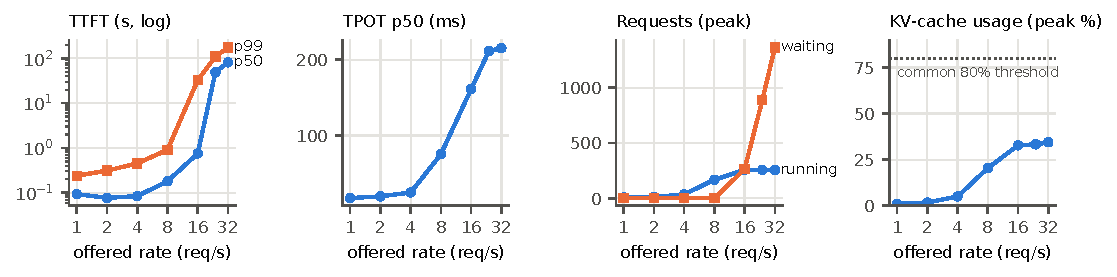
\includegraphics[width=\textwidth]{figures/fig_profile.pdf}
\caption{Measured single-replica behavior on a T4 (mean of three sessions; bands
show min--max). Requests and KV-cache usage are peaks of a 1\,Hz trace.}
\label{fig:profile}
\end{figure*}

\textbf{Capacity and the knee.} The three sessions agree closely: at every offered
rate, TTFT, TPOT and throughput differ by at most a few percent across sessions,
including across providers (Fig.~\ref{fig:profile}). Up to 8 requests/s all requests
are served with TTFT p99 below 1\,s (0.88--0.92\,s at 8 requests/s). At
16 requests/s, TTFT p99 rises to 32.2--33.0\,s. When the server is fully saturated
(24 and 32 requests/s offered) it completes 7.8--8.2 requests/s, which we take as
the single-replica capacity. TPOT grows with the running batch, from 17.5--17.9\,ms
at 1 request/s to about 215\,ms at saturation.

\textbf{What saturates first.} Past the knee, the number of running requests stops
at 256, the default \texttt{max\_num\_seqs}, and further requests wait; the peak
waiting count reaches 1{,}359--1{,}364 at 32 requests/s. KV-cache usage, by contrast,
peaks at 34.3--34.6\% even under the heaviest overload (32 requests/s). With these prompt and
output lengths, the server is limited by its scheduling cap and compute, not by
KV-cache memory: a KV-cache threshold of 80\%, a commonly suggested value, is
never reached by a single overloaded replica. KV-cache usage is not useless as a
signal; it rises monotonically with load (mean 9.1\% at 8 requests/s), but a
useful threshold for this workload is an order of magnitude below the common
default. Liu and Hu report the opposite regime for long contexts, where
KV-cache pressure dominates TTFT~\cite{liu2026decomposing}; together these suggest
that the right KV-cache threshold depends on the prompt-length distribution.

\textbf{Cold start.} A true first boot, which downloads the model and compiles
kernels, took 170\,s on Kaggle and 210\,s on Colab. Restarts with warm caches took
65.8--100.0\,s (six trials, median 73.4\,s), with no consistent ordering between
the first and second restart. Loading weights from disk took about 2\,s on Kaggle
and 6--12\,s on Colab. Cold start is therefore better described by a distribution
than a constant; we use the median warm value as the default replica startup time
and sweep it in simulation.

\section{Policy Comparison on the Emulated Cluster}
\label{sec:kind}
TODO(measured).

\section{Failure Mechanisms}
\label{sec:mechanisms}
TODO(measured).

\section{Sensitivity (Simulated)}
\label{sec:sweeps}
TODO(sim).

\section{Limitations}
\label{sec:limits}
\textbf{One small model on an older GPU.} All measurements use a 1.5B-parameter
model on a T4. Larger models, newer GPUs, tensor parallelism and
disaggregated prefill and decode change capacity, the batch at which latency
degrades, and cold-start time. The qualitative mechanisms we report (a
scheduling cap reached before KV-cache memory, backlog pinned to existing
replicas, startup delay that exceeds burst length) do not depend on these
numbers, but every threshold does.

\textbf{Approximate servers.} The policy comparison runs a real Kubernetes
control plane against an emulator, and the sweeps run a simulator. Both are
calibrated to the measured profile, and Table~\ref{tab:fidelity} reports where
each departs from it. The emulator applies one load factor to both prefill and
decode and therefore inflates TTFT near the knee; the simulator departs most at
16 requests/s, where a 60\,s measurement never reaches steady state. Neither
models preemption or prefix caching. We therefore emphasize relative
comparisons between policies and conclusions that hold in both tools.

\textbf{Laptop cluster.} The kind cluster is a single node on a laptop, so the
emulator's timing can be perturbed by other load; we kept the machine otherwise
idle during runs. Image pull time is excluded because the emulator image is
small and cached; a real vLLM image adds minutes to the first start on a node.

\textbf{Signals not evaluated.} We do not evaluate CPU- or GPU-utilization
policies. The emulator's CPU use does not resemble vLLM's, and our profiling
runs did not record GPU utilization. Prior guidance already cautions that
GPU utilization measures duty cycle rather than useful
work~\cite{gke2026autoscaling}.

\textbf{Synthetic workloads and routing.} Loads are synthetic Poisson processes
with lognormal lengths. Requests are routed by a Kubernetes Service, uniformly at
random across ready pods. A load-aware gateway would route around busy
replicas and change the backlog results.

\section{Artifact}
\label{sec:artifact}
TODO: repository URL.

\bibliographystyle{IEEEtran}
\bibliography{refs}
\end{document}
